\chapter{\label{chap:data}Data}

The stellar data selected for this project is a subset of the Gaia DR2 data-set~\cite{gaiaDr2}. This data, collected during the Gaia satellite mission~\cite{gaiaDr2}, is approximately \SI{500}{\giga\byte} and consists of a variety of parameters collected on a per-star basis. This is in great contrast with typical telescopic data which is primarily raw radiometric imagery and greatly expands the types of processing that may be conveniently applied. The subset of the parameters that are of interest to the pipeline are described in Section~\ref{sec:parameters}. As a result of hardware constraints, the investigation has been limited to a set of smaller regions from within the Gaia data-set. Four distinct areas were selected, bounded by by right ascension (\textit{RA}) $\times$ declination (\textit{Dec}), and represent regions of interest with varying stellar distributions. Table~\ref{tb:areas} sets out the cosmic ranges as well as the number of stars within these areas.

\begin{table}[H]
    \centering
    \caption{Areas Under Investigation}
    \label{tb:areas}
    \begin{tabular}{l c c c}
        \toprule
        Area & RA                        & Dec                       & Number of Stars \\
        \midrule
        A1   & \ang{120} up to \ang{246} & \ang{-2} up to \ang{60}   & \num{25486556}  \\
        A2   & \ang{295} up to \ang{308} & \ang{15} up to \ang{25}   & \num{23470239}  \\
        A3   & \ang{0} up to \ang{75}    & \ang{-90} up to \ang{-30} & \num{16781316}  \\
        A4   & \ang{0} up to \ang{45}    & \ang{30} up to \ang{70}   & \num{32333936}  \\
        \bottomrule
    \end{tabular}
\end{table}

\noindent \textit{Rationale for the choice of these four regions:}

\textbf{Area 1 (A1):}
This region was used in the precursor work of Mohammadi et al.~\cite{Mohammadi}.
It is the largest region of the four in terms of their span across RA and Dec.
Conversely, it also has the lowest density of stars across the region. This
results in large areas that contain very few stars. These \textit{dark} regions
are very apparent in Figure~\ref{fig:area1-scatter}. It contains several known
GCs, including a number in these \textit{dark} regions, which are expected to be
identified easily as they stand out from their dark and void stellar
surroundings.

\textbf{Area 2 (A2):}
The region was chosen because it is a much smaller area with a very high-density
of stars across the whole span. Additionally, it contains only one GC. This is
useful as a testing ground to see how the pipeline would handle regions
featuring a high amount of stars.

\textbf{Area 3 (A3):}
This area was also used in the paper by Mohammadi et al.\ and though its overall
density is less than for A2, it features specific regions with an extremely
high density of stars. Additionally, it contains 17 GCs, the Magellanic Clouds
(the name given to a specific pair of Dwarf galaxies), a supernova remnant, open
clusters, and galaxies. The Magellanic Clouds are the two extremely bright, very
densely packed regions that may be seen in Figure~\ref{fig:area3-scatter}. These
two very bright regions also contain some GCs and it would be useful to see
how the pipeline handles classifying these clusters with the interference of the
Magellanic clouds.

\textbf{Area 4 (A4):}
This area has no GCs, but contains the nearby and very bright Andromeda and Triangulum galaxies. These galaxies lie across the range of \ang{30}--\ang{50} Dec, and it would be illuminating to see if the pipeline detects them and classifies them as GCs. The remaining range, from \ang{50}--\ang{70} contains a large number of nebulae (large regions of very bright loosely-packed stellar gas).

\begin{figure}[H]
    \centering
    \begin{subfigure}[b]{0.49\textwidth}
        \includegraphics[width=\textwidth, height=0.4\textwidth]{scatterplots/area1-scatterplot.png}
        \caption{A1}
        \label{fig:area1-scatter}
    \end{subfigure}
    \begin{subfigure}[b]{0.49\textwidth}
        \includegraphics[width=\textwidth,height=0.8\textwidth]{scatterplots/area2-scatterplot.png}
        \caption{A2}
        \label{fig:area2-scatter}
    \end{subfigure}
    \begin{subfigure}[b]{0.49\textwidth}
        \includegraphics[width=\textwidth, height=0.8\textwidth]{scatterplots/area3-scatterplot.png}
        \caption{A3}
        \label{fig:area3-scatter}
    \end{subfigure}
    \begin{subfigure}[b]{0.49\textwidth}
        \includegraphics[width=\textwidth,height=0.8\textwidth]{scatterplots/area4-scatterplot.png}
        \caption{A4}
        \label{fig:area4-scatter}
    \end{subfigure}
    \caption{Stellar Distribution Heat-maps for the Four Areas}
    \label{fig:area-scatter}
\end{figure}

Figure~\ref{fig:area-scatter} depicts heat-maps of the four regions synthesized from the stellar information in the Gaia DR2 data-set. It provides an insight into the population and density of the stars found within the four areas. The brighter areas (yellow--white) contain more stars than the darker areas (red--black). From these heat-maps, the spots of increased stellar density are very evident. However, it is not immediately apparent whether these spots are GCs, Open Clusters (\textit{OC}), galaxies (\textit{Gal}), or some other stellar structure. Figure~\ref{fig:example-structures}, provides an example of some of these stellar structures for Area~1 and further highlights the difficulty in classifying these stellar structures by eye alone.

\begin{figure}[H]
    \centering
    \includegraphics[scale=0.25]{{scatterplots/area1-example-structures.pdf}}
    \begin{tabular}{r@{: }l r@{: }l r@{: }l}
        $\color{green}\circ{}$ & Open Clusters & $\color{blue}\circ{}$ & Globular Clusters   & $\color{cyan}\circ{}$ & Galaxies             \\
        \midrule
        OC1                    & Messier 44    & GC1                   & NGC4147             & Gal1                  & The Whirlpool Galaxy \\
        OC2                    & Messier 67    & GC2                   & NGC5024 and NGC5053 & Gal2                  & Malin 1
    \end{tabular}
    \caption{Stellar Structures Present in A1}
    \label{fig:example-structures}
\end{figure}

Area 1 contains more than the three GCs encircled in
Figure~\ref{fig:example-structures}. It contains an additional nine GCs (for a
total of 12), Area 2 contains just one known GC, and Area 3 contains 17
GCs~\cite{listGC, larger-list-gcs}. See Table~\ref{tb:known-gcs} for information
on the RA, the Dec, and the angular diameter (\textit{DIA}) for these globular
clusters where this information has been published. Note that the \textit{DIA}
is represented in arcminutes~(\si{\arcminute}) which is a measure of angular
distance where $\SI{1}{\arcminute} = \SI[quotient-mode=fraction]{1/60}{\degree}$
and is useful to provide an expectation of the size of a GC.

\begin{table}[H]
    \centering
    \caption{Known GCs}
    \label{tb:known-gcs}
    \begin{tabular}[t]{l l l c}
        \toprule
        \midrule
        \multicolumn{1}{c}{GC} & \ac{c}{RA (\si{\degree})}                 & \ac{c}{Dec (\si{\degree})}                  & DIA (\si{\arcminute}) \\
        \addlinespace[2em]
        \midrule[0.5pt]
        \multicolumn{4}{c}{Area 1}                                                                                                               \\
        \midrule[0.5pt]
        Palomar 3              & \ang[minimum-integer-digits=2]{151.38292} & \ang[minimum-integer-digits=2]{+00;04;18.0} & \ang{;1.6;}           \\
        Willman 1              & \ang[minimum-integer-digits=2]{162.35}    & \ang[minimum-integer-digits=2]{+51;03;00.0} & \ang{;7;}             \\
        Palomar 4              & \ang[minimum-integer-digits=2]{172.31999} & \ang[minimum-integer-digits=2]{+28;58;24.9} & \ang{;1.3;}           \\
        Koposov 1              & \ang[minimum-integer-digits=2]{179.82709} & \ang[minimum-integer-digits=2]{+12;15;36.0} & ---                   \\
        NGC 4147               & \ang[minimum-integer-digits=2]{182.52626} & \ang[minimum-integer-digits=2]{+18;32;33.5} & \ang{;4.4;}           \\
        NGC 5024               & \ang[minimum-integer-digits=2]{198.22945} & \ang[minimum-integer-digits=2]{+18;01;05.4} & \ang{;13;}            \\
        NGC 5053               & \ang[minimum-integer-digits=2]{199.11288} & \ang[minimum-integer-digits=2]{+17;42;00.5} & \ang{;10;}            \\
        M3                     & \ang[minimum-integer-digits=2]{205.54842} & \ang[minimum-integer-digits=2]{+28;22;38.2} & \ang{;18;}            \\
        NGC 5466               & \ang[minimum-integer-digits=2]{211.36371} & \ang[minimum-integer-digits=2]{+28;32;04.0} & \ang{;9;}             \\
        Palomar 5              & \ang[minimum-integer-digits=2]{229.02187} & \ang[minimum-integer-digits=2]{+00;06;41.8} & \ang{;8.0;}           \\
        M5                     & \ang[minimum-integer-digits=2]{229.63962} & \ang[minimum-integer-digits=2]{+02;04;54.9} & \ang{;21.6;}          \\
        GCI 38                 & \ang[minimum-integer-digits=2]{242.75247} & \ang[minimum-integer-digits=2]{+14;57;28.0} & \ang{;2.2;}           \\
        \addlinespace[2em]
        \midrule[0.5pt]
        \multicolumn{4}{c}{Area 2}                                                                                                               \\
        \midrule[0.5pt]
        M71                    & \ang[minimum-integer-digits=2]{298.44}    & \ang[minimum-integer-digits=2]{+18;46;45.1} & \ang{;7.2;}           \\
        \addlinespace[2em]
        \midrule[0.5pt]
        \multicolumn{4}{c}{Area 3}                                                                                                               \\
        \midrule[0.5pt]
        47 Tucanae             & \ang[minimum-integer-digits=2]{6.02363}   & \ang[minimum-integer-digits=2]{-72;04;52.6} & \ang{;50;}            \\
        NGC 121                & \ang[minimum-integer-digits=2]{6.70104}   & \ang[minimum-integer-digits=2]{-71;32;8.4}  & ---                   \\
        NGC 362                & \ang[minimum-integer-digits=2]{15.80942}  & \ang[minimum-integer-digits=2]{-70;50;55.6} & \ang{;14;}            \\
        NGC 1049               & \ang[minimum-integer-digits=2]{39.96875}  & \ang[minimum-integer-digits=2]{-34;16;08}   & ---                   \\
        NGC 1261               & \ang[minimum-integer-digits=2]{48.06754}  & \ang[minimum-integer-digits=2]{-55;12;59.2} & \ang{;6.85;}          \\
        NGC 1466               & \ang[minimum-integer-digits=2]{56.1375}   & \ang[minimum-integer-digits=2]{-71;40;17.0} & ---                   \\
        Arp Madore 1           & \ang[minimum-integer-digits=2]{58.76125}  & \ang[minimum-integer-digits=2]{-49;36;52.0} & ---                   \\
        NGC 1629               & \ang[minimum-integer-digits=2]{67.40417}  & \ang[minimum-integer-digits=2]{-71;50;18}   & ---                   \\
        NGC 1651               & \ang[minimum-integer-digits=2]{69.38625}  & \ang[minimum-integer-digits=2]{-70;35;08}   & ---                   \\
        NGC 1644               & \ang[minimum-integer-digits=2]{69.41500}  & \ang[minimum-integer-digits=2]{-66;11;49}   & ---                   \\
        NGC 1652               & \ang[minimum-integer-digits=2]{69.59542}  & \ang[minimum-integer-digits=2]{-68;40;23}   & ---                   \\
        NGC 1841               & \ang[minimum-integer-digits=2]{71.34625}  & \ang[minimum-integer-digits=2]{-83;59;49}   & ---                   \\
        NGC 1696               & \ang[minimum-integer-digits=2]{72.12500}  & \ang[minimum-integer-digits=2]{-68;14;35}   & ---                   \\
        NGC 1756               & \ang[minimum-integer-digits=2]{73.70792}  & \ang[minimum-integer-digits=2]{-69;14;15}   & ---                   \\
        NGC 1786               & \ang[minimum-integer-digits=2]{74.78291}  & \ang[minimum-integer-digits=2]{-67;44;43}   & ---                   \\
        NGC 1783               & \ang[minimum-integer-digits=2]{74.78667}  & \ang[minimum-integer-digits=2]{-65;59;07}   & ---                   \\
        NGC 1795               & \ang[minimum-integer-digits=2]{74.94583}  & \ang[minimum-integer-digits=2]{-69;48;05}   & ---                   \\
        \midrule
        \bottomrule
    \end{tabular}
\end{table}
It is these GCs that are used in the evaluation of the results of the pipeline.

\newpage

\section{\label{sec:parameters}The Parameters}

The Gaia DR2 data-set provides up to 88 parameters per star~\cite{gaiaDr2}. Of
these parameters, there are six that are required for the pipeline:

\begin{enumerate}
    \item Apparent Magnitude: This is a unitless quantity
          and is the measure of a star's brightness when observed from Earth (\NB{A higher apparent magnitude corresponds to a less bright star}). This is under the key \tx{phot_g_mean_mag} within the data-set.
    \item Right Ascension (\textit{RA}): This quantity is represented in degrees ($\degree$) and
          when coupled with the declination it provides a position for an astronomical
          body in the equatorial coordinate system. This is under the key \tx{ra}  within the data-set.
    \item Declination (\textit{Dec}): This quantity is represented in degrees ($\degree$) and
          when coupled with the right ascension it provides a position for an
          astronomical body in the equatorial coordinate system. This is under the key \tx{dec} within the data-set.
    \item Parallax: This quantity is measured in milliarcseconds
          (\si{\milliarcsecond}) and is the difference in the apparent position of an
          object when viewed along two different lines of sight~\cite{parallax}. This is under the key \tx{parallax}  within the data-set.
    \item Proper Motion of Right Ascension ($\text{PM}_{\text{RA}}$):
          Expressed in \si{\milliarcsecond\per\year} and is the motion of an
          astronomical body from the frame of the center of mass of the solar system in
          right ascension. This is under the key \tx{pmra} within the data-set.
    \item Proper Motion of Declination ($\text{PM}_{\text{Dec}}$): Expressed in
          \si{\milliarcsecond\per\year} and is the motion of an astronomical body from the frame of the center of mass of the solar system in declination. This is under the key \tx{pmdec} within the data-set.
\end{enumerate}
The details underlying the selection of these parameters alongside statistical analysis is provided in the sections that follow.

For the development of the pipeline, it is important to note, that the Gaia DR2
data-set does not include the parallax, $\text{PM}_{\text{RA}}$, or $\text{PM}_{\text{Dec}}$ for
\emph{all} stellar objects~\cite{GaiaDR2-parameters}. Additionally, the Gaia
data-set contains some spurious negative values for the
parallax~\cite{Luri2018}. Since these parameters are required for the pipeline,
the stars that are missing valid values for these parameters have been filtered out. The details on how many stars are filtered per area and the percentage
that remain are given in Table~\ref{tb:stars-with-no-parallax}.

\begin{table}[H]
    \centering
    \caption{\label{tb:stars-with-no-parallax} Filtered Stars}
    \begin{tabular}{c c c c c}
        \toprule
        Area & Total Number of Stars & Remaining Stars & Percentage Remaining \\
        \midrule
        A1   & \num{25 486 556}      & \num{17933864}  & 70.4\%               \\
        A2   & \num{23 470 239}      & \num{14268513}  & 60.8\%               \\
        A3   & \num{16 781 316}      & \num{9961034}   & 59.4\%               \\
        A4   & \num{32 333 936}      & \num{22243660}  & 68.8\%               \\
        \bottomrule
    \end{tabular}
\end{table}

\subsection{Apparent Magnitude}

The apparent magnitude provides information on the brightness of a star. In
isolation this is influenced by the mass of the star and the proximity of the
star to the observer. The closer the star is, the brighter it will appear. The
more massive the star, the higher its black-body radiation; thus, the more
energy it releases in the form of brighter light.

This parameter is used alongside, RA and Dec, to create the 2-dimensional
mapping that is fed into the Difference of Gaussian filters to detect blobs.
Histograms of the apparent magnitude across the four areas may be seen in
Figure~\ref{fig:areas-hist-magnitude}. Note that the frequency is presented on a
logarithmic axis and that a larger apparent magnitude corresponds to a less
bright star.
\begin{figure}[H]
    \centering
    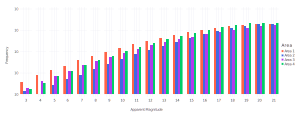
\includegraphics[width=\textwidth]{{julia/apparent-magnitude.pdf}}
    \caption{\label{fig:areas-hist-magnitude} Distribution of Apparent Magnitude Across the Four Areas}
\end{figure}
In Figure~\ref{fig:areas-hist-magnitude} it is apparent that as the stars grow dimmer, the distribution of stars between the four areas become more uniform.
It is also evident that Area 1 contains the most bright stars out of the four regions and that Area 2 contains the least amount of bright stars. However, this does not reveal the full story as each of the four areas contain a differing total number of stars. Thus, it is also necessary to consider the proportion of stars that lie within a specific apparent magnitude against the total number of stars contained within that area. This proportional distribution for each of the four areas may be seen in Figure~\ref{fig:areas-hist-magnitude:proportional}.

\begin{figure}[H]
    \centering
    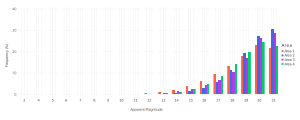
\includegraphics[width=\textwidth]{{julia/apparent-magnitude-proportional.pdf}}
    \caption{\label{fig:areas-hist-magnitude:proportional} Proportional Distribution of Apparent Magnitude Across the Four Areas}
\end{figure}
Figure~\ref{fig:areas-hist-magnitude:proportional} shows that the areas are predominantly composed of \textit{dim} stars. All four areas have at least \SI{50}{\percent} of their stars being of a magnitude of 19 or over.

\subsection{RA, Dec, and Distance (via Parallax)}

The RA and Dec are provided as part of the data-set and are easy to retrieve.
Together, these two quantities provide 2-dimensional spherical coordinates for a
star. However, two stars that may appear to overlap in terms of their RA and Dec
may be many thousands of light-years apart. Thus, to be able to effectively
cluster stars it is important to determine the third dimension representing the
distance from the Earth. By making use of trigonometry and the angular shifts
present in parallax, astronomers were able to determine a method to estimate the
distance of an object from the Earth. This distance is measured in parsecs and,
as may be seen in Figure~\ref{fig:stellar-parallax}, works by virtue of our
orbit around the Sun.
\begin{figure}[H]
    \centering
    \includegraphics[scale=0.37]{{img/Stellarparallax-parsec1.pdf}}
    \caption{\label{fig:stellar-parallax} Depiction of Parallax Measurement~\cite{parallax-img}}
\end{figure}
To determine the distance to some nearby star, we measure the angular
shift in the position of a distant star relative to the nearby star at opposite
points in our planet's orbit. This angular shift is the parallax and using this we may compute the distance in parsecs:
\begin{equation}
    \text{distance} = \frac{1}{\text{parallax}}
\end{equation}
The distributions of the parallax values across the four areas may be seen in the density plot in Figure~\ref{fig:areas-hist-parallax}.

\begin{figure}[H]
    \centering
    \includegraphics[width=0.9\textwidth]{julia/parallax.pdf}
    \caption{\label{fig:areas-hist-parallax} Distribution of Parallax Across the Four Areas}
\end{figure}

It is evident that the parallax values for the stars across the four regions span similar ranges and that they are all predominantly centered within \SI{0.01}{\milliarcsecond} to \SI{50.0}{\milliarcsecond}.

\subsection{Proper Motion}

It is also of interest to explore the spread of the data with respect to
\textit{proper motion of right ascension}, and \textit{proper motion of
    declination}. Together they describe the angular shift that a star experiences
over time, essentially representing the drift that the star is undergoing. In some cases this drift can be quite significant. Figure~\ref{fig:proper-motion} highlights this by showcasing the apparent shift in the position of Barnard's Star across the years 1991 to 2007.
\begin{figure}[H]
    \centering
    \includegraphics[width=0.40\textwidth, height=0.3\textwidth]{img/proper-motion.png}
    \caption{\label{fig:proper-motion} Proper Motion of Barnard’s Star from 1991--2007~\cite{pmra-img}}
\end{figure}
GCs are characterized by stars that are gravitationally bound to each other and are likely to be experiencing similar drift~\cite{Gratton}. Thus, the proper motion values provide a useful metric in identifying potential GCs. The Gaia data-set displays unprecedented accuracy in the proper motion values, with uncertainty in the range of~\cite{GaiaDR2-parameters}:
\begin{itemize}
    \item \SI{0.06}{\milliarcsecond\per\year} for apparent magnitudes < 15.
    \item \SI{0.2}{\milliarcsecond\per\year} for apparent magnitudes of 17.
    \item \SI{1.2}{\milliarcsecond\per\year} for apparent magnitudes of 20.
\end{itemize}
Density plots providing information on the distribution of $\text{PM}_{\text{RA}}$ and $\text{PM}_{\text{Dec}}$ may be
seen in Figure~\ref{fig:areas-hist-pm}.
\begin{figure}[H]
    \centering
    \includegraphics[width=\textwidth]{{julia/proper-motion.pdf}}
    \caption{\label{fig:areas-hist-pm} Distribution of Proper Motion Across the Four Areas}
\end{figure}

The plots show a great variety in the motion of the stars. It is evident that the motion of $\text{PM}_{\text{RA}}$ is larger than $\text{PM}_{\text{Dec}}$ for all areas. Additionally, the stars within Area 2 are experiencing drift within a tighter bound for both $\text{PM}_{\text{RA}}$ and $\text{PM}_{\text{Dec}}$ when compared to the other areas. The remaining three areas share a similar distribution in their stellar motion for RA, but Area 4 seems to have less drift in Dec than either Area 1 or Area 3. The largest movement in the direction of $\text{RA}$ is in Area 3 with \SI{5750}{\milliarcsecond\per\year}, and the largest movement in the $\text{Dec}$ is in Area 1 with \SI{1350}{\milliarcsecond\per\year}.
